% 若编译失败,且生成 .synctex(busy) 辅助文件,可能有两个原因:
% 1. 需要插入的图片不存在:Ctrl + F 搜索 'figure' 将这些代码注释/删除掉即可
% 2. 路径/文件名含中文或空格:更改路径/文件名即可

% --------------------- 文章宏包及相关设置 --------------------- %
% >> ------------------ 文章宏包及相关设置 ------------------ << %
% 设定文章类型与编码格式
\documentclass[UTF8]{article}		

% 物理实验报告所需的其它宏包
\usepackage{ulem}   % \uline 下划线支持
\usepackage{circuitikz} % 电路图 tikz 支持
\usepackage{pdfpages}   % 用于导入 pdf 文件

% 本 .tex 专属的宏定义
    \def\V{\ \mathrm{V}}
    \def\uV{\ \mu\mathrm{V}}
    \def\mV{\ \mathrm{mV}}
    \def\K{\ \mathrm{K}}
    \def\kV{\ \mathrm{KV}}
    \def\KV{\ \mathrm{KV}}
    \def\MV{\ \mathrm{MV}}
    \def\uA{\ \mu\mathrm{A}}
    \def\mA{\ \mathrm{mA}}
    \def\A{\ \mathrm{A}}
    \def\kA{\ \mathrm{KA}}
    \def\KA{\ \mathrm{KA}}
    \def\MA{\ \mathrm{MA}}
    \def\O{\ \Omega}
    \def\mO{\ \Omega}
    \def\kO{\ \mathrm{K}\Omega}
    \def\KO{\ \mathrm{K}\Omega}
    \def\MO{\ \mathrm{M}\Omega}
    \def\Hz{\ \mathrm{Hz}}
    \def\uF{\ \mu\mathrm{F}}
    \def\mF{\ \mathrm{mF}}
    \def\F{\ \mathrm{F}}

% 自定义宏定义
    \def\N{\mathbb{N}}
    \def\F{\mathbb{F}}
    \def\Z{\mathbb{Z}}
    \def\Q{\mathbb{Q}}
    \def\R{\mathbb{R}}
    \def\C{\mathbb{C}}
    \def\T{\mathbb{T}}
    \def\S{\mathbb{S}}
    %\def\A{\mathbb{A}}
    \def\I{\mathscr{I}}
    \def\d{\mathrm{d}}
    \def\p{\partial}


% 导入基本宏包
    \usepackage[UTF8]{ctex}     % 设置文档为中文语言
    \usepackage{hyperref}  % 宏包:自动生成超链接 (此宏包与标题中的数学环境冲突)
    \hypersetup{
        colorlinks=true,    % false:边框链接 ; true:彩色链接
        citecolor={blue},    % 文献引用颜色
        linkcolor={blue},   % 目录 (我们在目录处单独设置),公式,图表,脚注等内部链接颜色
        urlcolor={orange},    % 网页 URL 链接颜色,包括 \href 中的 text
        % cyan 浅蓝色 
        % magenta 洋红色
        % yellow 黄色
        % black 黑色
        % white 白色
        % red 红色
        % green 绿色
        % blue 蓝色
        % gray 灰色
        % darkgray 深灰色
        % lightgray 浅灰色
        % brown 棕色
        % lime 石灰色
        % olive 橄榄色
        % orange 橙色
        % pink 粉红色
        % purple 紫色
        % teal 蓝绿色
        % violet 紫罗兰色
    }
    % \usepackage{docmute}    % 宏包:子文件导入时自动去除导言区,用于主/子文件的写作方式,\include{./51单片机笔记}即可。注:启用此宏包会导致.tex文件capacity受限。
    \usepackage{amsmath}    % 宏包:数学公式
    \usepackage{mathrsfs}   % 宏包:提供更多数学符号
    \usepackage{amssymb}    % 宏包:提供更多数学符号
    \usepackage{pifont}     % 宏包:提供了特殊符号和字体
    \usepackage{extarrows}  % 宏包:更多箭头符号 
    \usepackage{multicol}   % 宏包:支持多栏 

% 文章页面margin设置
    \usepackage[a4paper]{geometry}
        \geometry{top=0.75in}
        \geometry{bottom=0.75in}
        \geometry{left=0.75in}
        \geometry{right=0.75in}   % 设置上下左右页边距
        \geometry{marginparwidth=1.75cm}    % 设置边注距离(注释、标记等)

% 配置数学环境
    \usepackage{amsthm} % 宏包:数学环境配置
    % theorem-line 环境自定义
        \newtheoremstyle{MyLineTheoremStyle}% <name>
            {11pt}% <space above>
            {11pt}% <space below>
            {\kaishu}% <body font> 默认使用正文字体, \kaishu 为楷体
            {}% <indent amount>
            {\bfseries}% <theorem head font> 设置标题项为加粗
            {:\ \ }% <punctuation after theorem head>
            {.5em}% <space after theorem head>
            {\textbf{#1}\thmnumber{#2}\ \ (\,\textbf{#3}\,)}% 设置标题内容顺序
        \theoremstyle{MyLineTheoremStyle} % 应用自定义的定理样式
        \newtheorem{LineTheorem}{Theorem.\,}
    % theorem-block 环境自定义
        \newtheoremstyle{MyBlockTheoremStyle}% <name>
            {11pt}% <space above>
            {11pt}% <space below>
            {\kaishu}% <body font> 使用默认正文字体
            {}% <indent amount>
            {\bfseries}% <theorem head font> 设置标题项为加粗
            {:\\ \indent}% <punctuation after theorem head>
            {.5em}% <space after theorem head>
            {\textbf{#1}\thmnumber{#2}\ \ (\,\textbf{#3}\,)}% 设置标题内容顺序
        \theoremstyle{MyBlockTheoremStyle} % 应用自定义的定理样式
        \newtheorem{BlockTheorem}[LineTheorem]{Theorem.\,} % 使用 LineTheorem 的计数器
    % definition 环境自定义
        \newtheoremstyle{MySubsubsectionStyle}% <name>
            {11pt}% <space above>
            {11pt}% <space below>
            {}% <body font> 使用默认正文字体
            {}% <indent amount>
            {\bfseries}% <theorem head font> 设置标题项为加粗
            {:\\ \indent}% <punctuation after theorem head>
            {0pt}% <space after theorem head>
            {\textbf{#3}}% 设置标题内容顺序
        \theoremstyle{MySubsubsectionStyle} % 应用自定义的定理样式
        \newtheorem{definition}{}

%宏包:有色文本框(proof环境)及其设置
    \usepackage{xcolor}    %设置插入的文本框颜色
    \usepackage[strict]{changepage}     % 提供一个 adjustwidth 环境
    \usepackage{framed}     % 实现方框效果
        \definecolor{graybox_color}{rgb}{0.95,0.95,0.96} % 文本框颜色。修改此行中的 rgb 数值即可改变方框纹颜色,具体颜色的rgb数值可以在网站https://colordrop.io/ 中获得。(截止目前的尝试还没有成功过,感觉单位不一样)(找到喜欢的颜色,点击下方的小眼睛,找到rgb值,复制修改即可)
        \newenvironment{graybox}{%
        \def\FrameCommand{%
        \hspace{1pt}%
        {\color{gray}\vrule width 2pt}%
        {\color{graybox_color}\vrule width 4pt}%
        \colorbox{graybox_color}%
        }%
        \MakeFramed{\advance\hsize-\width\FrameRestore}%
        \noindent\hspace{-4.55pt}% disable indenting first paragraph
        \begin{adjustwidth}{}{7pt}%
        \vspace{2pt}\vspace{2pt}%
        }
        {%
        \vspace{2pt}\end{adjustwidth}\endMakeFramed%
        }

% 外源代码插入设置
    % matlab 代码插入设置
    \usepackage{matlab-prettifier}
        \lstset{style=Matlab-editor}    % 继承 matlab 代码高亮 , 此行不能删去
    \usepackage[most]{tcolorbox} % 引入tcolorbox包 
    \usepackage{listings} % 引入listings包
        \tcbuselibrary{listings, skins, breakable}
        \newfontfamily\codefont{Consolas} % 定义需要的 codefont 字体
        \lstdefinestyle{MatlabStyle_inc}{   % 插入代码的样式
            language=Matlab,
            basicstyle=\footnotesize\ttfamily\codefont,    % ttfamily 确保等宽 
            breakatwhitespace=false,
            breaklines=true,
            captionpos=b,
            keepspaces=true,
            numbers=left,
            numbersep=15pt,
            showspaces=false,
            showstringspaces=false,
            showtabs=false,
            tabsize=2,
            xleftmargin=15pt,   % 左边距
            %frame=single, % single 为包围式单线框
            frame=shadowbox,    % shadowbox 为带阴影包围式单线框效果
            %escapeinside=``,   % 允许在代码块中使用 LaTeX 命令 (此行无用)
            %frameround=tttt,    % tttt 表示四个角都是圆角
            framextopmargin=0pt,    % 边框上边距
            framexbottommargin=0pt, % 边框下边距
            framexleftmargin=5pt,   % 边框左边距
            framexrightmargin=5pt,  % 边框右边距
            rulesepcolor=\color{red!20!green!20!blue!20}, % 阴影框颜色设置
            %backgroundcolor=\color{blue!10}, % 背景颜色
        }
        \lstdefinestyle{MatlabStyle_src}{   % 插入代码的样式
            language=Matlab,
            basicstyle=\small\ttfamily\codefont,    % ttfamily 确保等宽 
            breakatwhitespace=false,
            breaklines=true,
            captionpos=b,
            keepspaces=true,
            numbers=left,
            numbersep=15pt,
            showspaces=false,
            showstringspaces=false,
            showtabs=false,
            tabsize=2,
        }
        \newtcblisting{matlablisting}{
            %arc=2pt,        % 圆角半径
            % 调整代码在 listing 中的位置以和引入文件时的格式相同
            top=0pt,
            bottom=0pt,
            left=-5pt,
            right=-5pt,
            listing only,   % 此句不能删去
            listing style=MatlabStyle_src,
            breakable,
            colback=white,   % 选一个合适的颜色
            colframe=black!0,   % 感叹号后跟不透明度 (为 0 时完全透明)
        }
        \lstset{
            style=MatlabStyle_inc,
        }

% table 支持
    \usepackage{booktabs}   % 宏包:三线表
    \usepackage{tabularray} % 宏包:表格排版
    \usepackage{longtable}  % 宏包:长表格

% figure 设置
    \usepackage{graphicx}  % 支持 jpg, png, eps, pdf 图片 
    \usepackage{svg}       % 支持 svg 图片
        \svgsetup{
            % 指向 inkscape.exe 的路径
            inkscapeexe = C:/aa_MySame/inkscape/bin/inkscape.exe, 
            % 一定程度上修复导入后图片文字溢出几何图形的问题
            inkscapelatex = false                 
        }
    \usepackage{subcaption} % 用于子图和小图注  

% 图表进阶设置
    \usepackage{caption}    % 图注、表注
        \captionsetup[figure]{name=图}  
        \captionsetup[table]{name=表}
        \captionsetup{
            labelfont=bf, % 设置标签为粗体
            textfont=bf,  % 设置文本为粗体
            font=small  
        }
    \usepackage{float}     % 图表位置浮动设置 
    \usepackage{etoolbox} % 用于保证图注表注的数学字符为粗体
        \AtBeginEnvironment{figure}{\boldmath} % 图注中的数学字符为粗体
        \AtBeginEnvironment{table}{\boldmath}  % 表注中的数学字符为粗体
        \AtBeginEnvironment{tabular}{\unboldmath}   % 保证表格中的数学字符不受额外影响

% 圆圈序号自定义
    \newcommand*\circled[1]{\tikz[baseline=(char.base)]{\node[shape=circle,draw,inner sep=0.8pt, line width = 0.03em] (char) {\bfseries #1};}}   % TikZ solution

% 列表设置
    \usepackage{enumitem}   % 宏包:列表环境设置
        \setlist[enumerate]{
            label=(\arabic*) ,   % 设置序号样式为加粗的 (1) (2) (3)
            ref=\arabic*, % 如果需要引用列表项,这将决定引用格式(这里仍然使用数字)
            itemsep=0pt, parsep=0pt, topsep=0pt, partopsep=0pt, leftmargin=3.5em} 
        \setlist[itemize]{itemsep=0pt, parsep=0pt, topsep=0pt, partopsep=0pt, leftmargin=3.5em}
        \newlist{circledenum}{enumerate}{1} % 创建一个新的枚举环境  
        \setlist[circledenum,1]{  
            label=\protect\circled{\arabic*}, % 使用 \arabic* 来获取当前枚举计数器的值,并用 \circled 包装它  
            ref=\arabic*, % 如果需要引用列表项,这将决定引用格式(这里仍然使用数字)
            itemsep=0pt, parsep=0pt, topsep=0pt, partopsep=0pt, leftmargin=3.5em
        }  

% 其它设置
    % 脚注设置
        \renewcommand\thefootnote{\ding{\numexpr171+\value{footnote}}}
    % 参考文献引用设置
        \bibliographystyle{unsrt}   % 设置参考文献引用格式为unsrt
        \newcommand{\upcite}[1]{\textsuperscript{\cite{#1}}}     % 自定义上角标式引用
    % 文章序言设置
        \newcommand{\cnabstractname}{序言}
        \newenvironment{cnabstract}{%
            \par\Large
            \noindent\mbox{}\hfill{\bfseries \cnabstractname}\hfill\mbox{}\par
            \vskip 2.5ex
            }{\par\vskip 2.5ex}

% 文章默认字体设置
    \usepackage{fontspec}   % 宏包:字体设置
        \setmainfont{SimSun}    % 设置中文字体为宋体字体
        \setCJKmainfont[AutoFakeBold=3]{SimSun} % 设置加粗字体为 SimSun 族,AutoFakeBold 可以调整字体粗细
        \setmainfont{Times New Roman} % 设置英文字体为Times New Roman

% 各级标题自定义设置
    \usepackage{titlesec}   
        % section标题自定义设置 
        \titleformat{\section}[hang]{\normalfont\Large\bfseries\boldmath}{\thesection}{8pt}{}
        % subsection 标题自定义设置
        \titleformat{\subsection}[hang]{\normalfont\large\bfseries\boldmath}{\thesubsection}{8pt}{}
        \titlespacing*{\subsection}{0pt}{6pt}{3pt} % 控制上下间距


% --------------------- 文章宏包及相关设置 --------------------- %
% >> ------------------ 文章宏包及相关设置 ------------------ << %


% ------------------------ 文章信息区 ------------------------ %
% ------------------------ 文章信息区 ------------------------ %
% 页眉页脚设置
\usepackage{fancyhdr}   %宏包:页眉页脚设置
    \pagestyle{fancy}
    \fancyhf{}
    \cfoot{\thepage}
    \renewcommand\headrulewidth{1pt}
    \renewcommand\footrulewidth{0pt}
    \rhead{\bfseries \large {\color{red} 分组序号: 2-05}}    
    \chead{《基础物理实验》实验报告,\ 丁毅,\ 2023K8009908031}
    \lhead{Ex.9 微波干涉 (2024.10.27)}

% 开始编辑文章

\begin{document}
\begin{center}\large
    \vspace*{-0.8cm}
    \noindent{\huge\bfseries《\ \ 基\ \ 础\ \ 物\ \ 理\ \ 实\ \ 验\ \ \ 》\ \ 实\ \ 验\ \ 报\ \ 告 }
    \\\vspace{0.1cm}
    \noindent{
    {\bfseries 
    实验名称:\uline{\hspace{2cm} 微波布拉格衍射 \hspace{2cm}}
    }\hspace{0.4cm}
    指导教师:\uline{\hspace{0.3cm}易栖如\ \ yiqiru@ucas.ac.cn\hspace{0.3cm}}
    }
    \\\vspace{0.1cm}
    \noindent
    {
    姓名:\uline{\,\,\,丁毅\,\,\,}\hspace{0.2cm}
    学号:\uline{\,\,\,{ 2023K8009908031}\,\,\,}\hspace{0.2cm}
    班级/专业:\uline{\,\,\,{2308/电子信息}\,\,\,}\hspace{0.2cm}
    分组序号:\uline{\,\,\,{2-05}\,\,\,}
    }
    \\\vspace{0.1cm}
    \noindent{
    实验日期:\uline{\,\,{ 2024.10.27}\,\,}\hspace{0.2cm}
    实验地点:\uline{\,\,\,教学楼{ 717}\,\,\,}\hspace{0.2cm}
    是否调课/补课:\uline{\hspace{0.26cm}否 \hspace{0.26cm}}\hspace{0.2cm}
    成绩:\uline{\hspace{2cm}}
    }
\end{center}
\vspace{-0.4cm}
\noindent\rule{\textwidth}{0.075em}   % 分割线
\vspace{-1.0cm}
% ------------------------ 文章信息区 ------------------------ %
% ------------------------ 文章信息区 ------------------------ %


% 目录
\setcounter{tocdepth}{3}  % 目录深度为 2(不显示 subsubsection)
\noindent\tableofcontents\thispagestyle{fancy}   % 显示页码、页眉等

\newpage
\rhead{\bfseries 分组序号: 2-05}

\section{实验目的}
1.了解与学习微波产生的基本原理以及传播和接收等基本特性;

2.观测微波衍射、干涉等实验现象;

3.观测模拟晶体的微波布拉格衍射现象;

4.通过迈克尔逊实验观测微波波长。

\section{实验器材}
DHMS-1型微波光学综合实验仪一套,包括:X波段微波信号源、微波发生器、发射喇叭、接收喇叭、微波检波器、检波信号数字显示器、可旋转载物平台和支架,以及实验用附件(反射板、分束板、单缝板、双缝板、晶体模型、读数机构等)。

\section{实验原理}
微波波长从1\,m到0.1\,mm,其频率范围为$ 300\,\mathrm{MHz}\sim3000\,\mathrm{GHz} $,是无线电波中波长最短的电磁波。微波波长介于一般无线电波与光波之间,因此它不仅具有无线电波的性质,还具有光波的性质,即具有光的直线传播、反射、折射、衍射、干涉等性质。微波波长与普通电磁波相比要短得多,因此其反射、辐射、传播和接收器件都有自己的特殊性;同时,它的波长又比X射线、光波长得多,故而用微波来仿真“晶格”衍射,发生明显衍射效应的“晶格”可以放大到宏观的尺度。

\subsection{微波的产生和接收}
本次实验中所使用的微波发生器采用电调制方法实现。微波发生器内部有一个电压可调控制的VCO,用于产生一个$ 4.4\,\mathrm{GHz}\sim 5.2\,\mathrm{GHz} $的信号,它的输出频率可以随输入电压的不同作相应改变,经过滤波器后取二次谐波$ 8.8\,\mathrm{GHz}\sim9.8\,\mathrm{GHz} $,经过衰减器作适当的衰减后,再放大,经过隔离器后,通过探针输出至波导口,再通过E面天线发射出去。

接收部分采用检波/数显一体化设计。由E面喇叭天线接收微波信号,传给高灵敏度的检波管后转化为电信号,通过穿心电容送出检波电压,再通过A/D转换(即模-数转换,Anglog-Digital),由液晶显示器显示微波相对强度。

\subsection{微波的单缝衍射实验}
当一平面微波入射到一宽度和微波波长可比拟的一狭缝时,在缝后会发生如光波一般的衍射现象,其示意图与强度分布如图 \ref{fig-single} 所示。

\begin{figure}[H]
    \centering
    \begin{tikzpicture}
        \draw (-6.2,0)--(6.2,0);
        \draw (0,0)--(0,5);
        \node [below] at(-6,0) {$ \frac{-3a\sin\varphi}{\lambda} $};
        \node [below] at(-4,0) {$ \frac{-2a\sin\varphi}{\lambda} $};
        \node [below] at(-2,0) {$ \frac{-a\sin\varphi}{\lambda} $};
        \node [below] at(2,0) {$ \frac{a\sin\varphi}{\lambda} $};
        \node [below] at(4,0) {$ \frac{2a\sin\varphi}{\lambda} $};
        \node [below] at(6,0) {$ \frac{3a\sin\varphi}{\lambda} $};
        \node at(0,-0.5) {0};
        \draw [very thick,domain=-6:-0.01,samples=100] plot (\x,{5*pow(sin(\x*pi/2 r)/(\x*pi/2),2)});
        \draw [very thick,domain=0.01:6,samples=100] plot (\x,{5*pow(sin(\x*pi/2 r)/(\x*pi/2),2)});
        \draw [very thick] (0.01,5)--(-0.01,5);
        
        \draw (-10,2)--(-9.5,2)--(-9.5,1.8)--(-11,1.8)--(-11,2)--(-10,2);
        \draw (-8,2)--(-8.5,2)--(-8.5,1.8)--(-7,1.8)--(-7,2)--(-8,2);
        \draw [thick,<-] (-9.5,2)--(-9.5,4);
        \draw [thick,<-] (-8.5,2)--(-8.5,4);
        \draw [thick] (-9.5,2)--(-9.5,1.8);
        \draw [thick] (-8.5,2)--(-8.5,1.8);
        \draw [dashed] (-9.5,1.8)--(-9.5,-1);
        \draw [dashed] (-8.5,1.8)--(-8.5,-1);
        \draw [thick,->] (-9.5,1.8)--(-9,0);
        \draw [thick,->] (-8.5,1.8)--(-8,0);
        \draw [<->] (-9.5,-0.5)--(-8.5,-0.5);
        %\draw (-8.5,0.5) to[out=0,in=210]  (-8.16,0.6);
        \draw (-8.5,0.5) arc (270:285:1.3);
        
        \node [below] at(-9,-0.5) {$ a $};
        \node [below] at(-8.3,0.5) {$ \theta $};
    \end{tikzpicture}
    \caption{单缝衍射示意图与强度分布}
    \label{fig-single}
\end{figure}

如为一维衍射,微波单缝衍射图样的强度分布规律为
\[I=I_0\frac{\sin^2\mu}{\mu^2}\qquad\left(\mu=\frac{\pi a\sin\theta}{\lambda}\right)\]
其中$ I_0 $为中央主极大中心的微波强度,$ a $为单缝的宽度,$ \lambda $是微波的波长,$ \theta $为衍射角。与光的单缝衍射一样,当$ a\sin\theta=\pm k\lambda\,(k=1,2,3,\cdots) $时,相应的$ \theta $角位置衍射强度为0。如测出衍射强度分布则可依据第一级衍射最小值所对应的$ \theta $,求出微波波长$ \lambda=a\sin\theta $.

\subsection{微波的双缝干涉实验}
当一平面波垂直入射到一金属板的两条狭缝上,狭缝就成为次级波波源。由两缝发出的次级波是相干波,因此在金属板的背后空间中,将产生干涉现象。由于波通过每个缝都有衍射现象,因此实验将是干涉与衍射两者结合的结果。为了只研究主要来自两缝中央衍射波相互干涉的结果,令双缝的缝宽$ a $接近$ \lambda $。当两缝之间的间隔$ b $较大时,干涉强度受单缝衍射的影响小;当$ b $较大时,干涉强度受单缝衍射影响大。干涉加强的角度为
\[\varphi=\arcsin\left(\frac{k\lambda}{a+b}\right)\qquad k=1,2,3,\cdots\]
干涉减弱的角度为
\[\varphi=\arcsin\left(\frac{2k+1}{2}\cdot\frac{\lambda}{a+b}\right)\qquad k=1,2,3,\cdots\]

\subsection{微波的迈克尔逊干涉实验}
1881年物理学家迈克尔逊与莫雷合作,为研究“以太”漂移而设计制造了利用分振幅法产生双光束以实现干涉的迈克尔逊干涉仪。

\begin{figure}[H]\centering
\includegraphics[width=0.85\columnwidth]{assets/迈克尔逊干涉仪.pdf}
\caption{迈克尔逊干涉仪}\label{迈克尔逊干涉仪}
\end{figure}

迈克尔逊干涉仪如图 \ref{迈克尔逊干涉仪} 所示,图中反射镜 $M_1$ 与 $M_2'$(虚镜)水平(此时的干涉现象类似等倾干涉),下方是接收屏或接受仪,图中的虚线光路表示出射向无穷远处(不被观察屏接收),或振幅较小而可以忽略的光线。

可以证明,从出射开始,分束所得到的两束光的空间光程差为 $\Delta l = 2 d \cos \theta$,其中 $\theta$ 是光束射向反射镜 $M$ 的入射角(光源平行出射时,$\theta = 0$),再考虑上在分束镜 $G$ 处发生的相位突变(半波损失),得到总光程差 $\Delta L = 2 d \cos \theta + \frac{\lambda}{2}$。
\begin{align}
\begin{matrix}
\displaystyle \text{OPD: }& \Delta L = 2 d \cos \theta + \frac{\lambda}{2} \\ 
\displaystyle \text{亮条纹:}&\Delta L = k \lambda \Longrightarrow \cos \theta_k = \frac{\lambda}{2 n_f d} \cdot (k - \frac{1}{2}),\quad k = 1, 2, 3, ... \\ 
\displaystyle \text{暗条纹:}&\Delta L = (k + \frac{1}{2}) \lambda \Longrightarrow \cos \theta_k = \frac{\lambda}{2 n_f d} \cdot k,\quad k = 0, 1, 2, 3, ...\\ 
\displaystyle \text{条纹间距:}& | \Delta r | \propto  \frac{\lambda}{2d \sin \theta_k}
\end{matrix}
\end{align}
迈克尔逊干涉是一种特殊的等倾干涉,干涉条纹内疏外密。

特别地,在本实验中,我们只测量中心处一点的亮暗情况。固定其中一个反射板,并移动另一块反射板,设两个相邻极小(大)值之间,反射板移动了距离 $x$,则有 $2x = \lambda$。由此可知,从第一个极小(大)值开始,设第 $N$ 次达到极小(大)值时,金属板移动了 $L$,则有:
\begin{equation}
    2L = N\lambda \Longrightarrow \lambda = \frac{2L}{N}
\end{equation}

\subsection{微波布拉格衍射}
\subsubsection{晶体结构}
组成晶体的原子或分子会按一定规律在空间内周期性排列。其中最简单的结构,是组成晶体的原子在直角坐标中沿$ x,y,z $三个方向,按固定的距离$ a $(晶格常数)在空间依序重复排列,形成简单的立方点阵。

\begin{figure}[h]
    \centering
    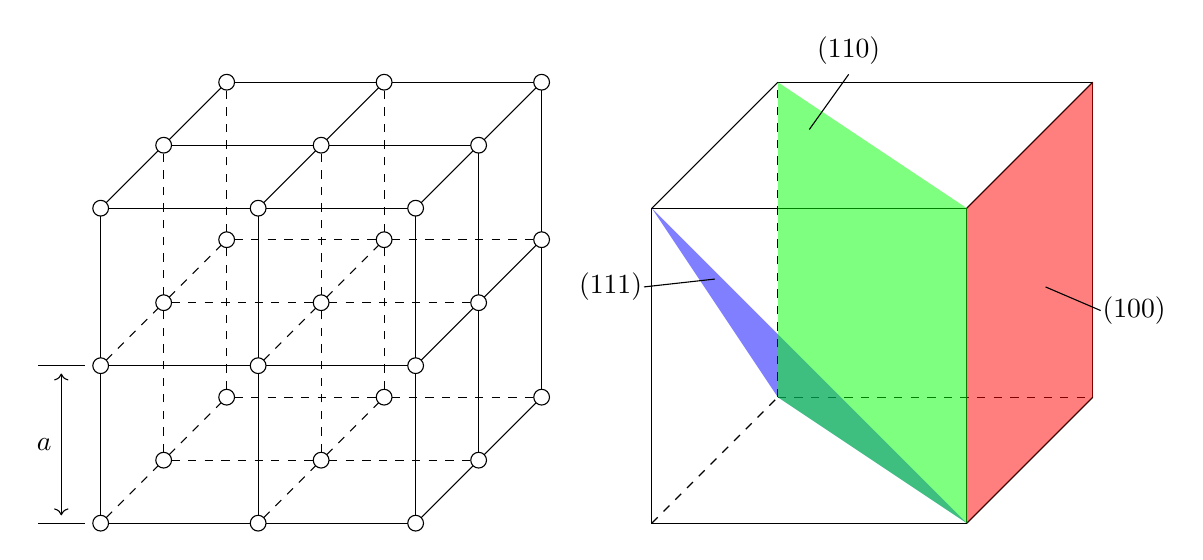
\begin{tikzpicture}
        \draw (0,0) circle [radius=0.1];
        \draw (2,0) circle [radius=0.1];
        \draw (4,0) circle [radius=0.1];
        \draw (4,2) circle [radius=0.1];
        \draw (4,4) circle [radius=0.1];
        \draw (0,2) circle [radius=0.1];
        \draw (0,4) circle [radius=0.1];
        \draw (2,2) circle [radius=0.1];
        \draw (2,4) circle [radius=0.1];
        \draw (0.8,0.8) circle [radius=0.1];
        \draw (0.8,2.8) circle [radius=0.1];
        \draw (0.8,4.8) circle [radius=0.1];
        \draw (2.8,0.8) circle [radius=0.1];
        \draw (4.8,0.8) circle [radius=0.1];
        \draw (2.8,2.8) circle [radius=0.1];
        \draw (2.8,4.8) circle [radius=0.1];
        \draw (4.8,2.8) circle [radius=0.1];
        \draw (4.8,4.8) circle [radius=0.1];				
        \draw (1.6,1.6) circle [radius=0.1];				
        \draw (3.6,1.6) circle [radius=0.1];				
        \draw (5.6,1.6) circle [radius=0.1];				
        \draw (1.6,3.6) circle [radius=0.1];				
        \draw (1.6,5.6) circle [radius=0.1];				
        \draw (3.6,3.6) circle [radius=0.1];				
        \draw (3.6,5.6) circle [radius=0.1];				
        \draw (5.6,3.6) circle [radius=0.1];				
        \draw (5.6,5.6) circle [radius=0.1];
        
        \draw (0.1,0)--(1.9,0);
        \draw (0,0.1)--(0,1.9);
        \draw (0,2.1)--(0,3.9);
        \draw (2.1,0)--(3.9,0);
        \draw (0.1,2)--(1.9,2);
        \draw (0.1,4)--(1.9,4);
        \draw (2.1,2)--(3.9,2);
        \draw (2.1,4)--(3.9,4);
        \draw (2,0.1)--(2,1.9);
        \draw (4,0.1)--(4,1.9);
        \draw (2,2.1)--(2,3.9);
        \draw (4,2.1)--(4,3.9);
        \draw [dashed] (0.8,0.9)--(0.8,2.7);
        \draw [dashed] (2.8,0.9)--(2.8,2.7);
        \draw (4.8,0.9)--(4.8,2.7);
        \draw [dashed] (0.9,0.8)--(2.7,0.8);
        \draw [dashed] (0.9,2.8)--(2.7,2.8);
        \draw (0.9,4.8)--(2.7,4.8);
        \draw [dashed] (0.8,2.9)--(0.8,4.7);
        \draw [dashed] (2.8,2.9)--(2.8,4.7);
        \draw (4.8,2.9)--(4.8,4.7);
        \draw [dashed] (2.9,0.8)--(4.7,0.8);
        \draw [dashed] (2.9,2.8)--(4.7,2.8);
        \draw (2.9,4.8)--(4.7,4.8);
        \draw [dashed] (1.6,1.7)--(1.6,3.5);
        \draw [dashed] (3.6,1.7)--(3.6,3.5);
        \draw (5.6,1.7)--(5.6,3.5);
        \draw [dashed] (1.6,3.7)--(1.6,5.5);
        \draw [dashed] (3.6,3.7)--(3.6,5.5);
        \draw (5.6,3.7)--(5.6,5.5);
        \draw [dashed] (1.7,1.6)--(3.5,1.6);
        \draw [dashed] (1.7,3.6)--(3.5,3.6);
        \draw (1.7,5.6)--(3.5,5.6);
        \draw [dashed] (3.7,1.6)--(5.5,1.6);
        \draw [dashed] (3.7,3.6)--(5.5,3.6);
        \draw (3.7,5.6)--(5.5,5.6);				
        \draw [dashed] (0.07,0.07)--(0.73,0.73);
        \draw [dashed] (0.07,2.07)--(0.73,2.73);
        \draw (0.07,4.07)--(0.73,4.73);				
        \draw [dashed] (2.07,0.07)--(2.73,0.73);
        \draw [dashed] (2.07,2.07)--(2.73,2.73);
        \draw (2.07,4.07)--(2.73,4.73);				
        \draw (4.07,0.07)--(4.73,0.73);
        \draw (4.07,2.07)--(4.73,2.73);
        \draw (4.07,4.07)--(4.73,4.73);				
        \draw [dashed] (0.87,0.87)--(1.53,1.53);
        \draw [dashed] (0.87,2.87)--(1.53,3.53);
        \draw (0.87,4.87)--(1.53,5.53);				
        \draw [dashed] (2.87,0.87)--(3.53,1.53);
        \draw [dashed] (2.87,2.87)--(3.53,3.53);
        \draw (2.87,4.87)--(3.53,5.53);				
        \draw (4.87,0.87)--(5.53,1.53);
        \draw (4.87,2.87)--(5.53,3.53);
        \draw (4.87,4.87)--(5.53,5.53);
        \draw (-0.2,0)--(-0.8,0);				
        \draw (-0.2,2)--(-0.8,2);
        \draw [<->](-0.5,0.1)--(-0.5,1.9);
        \node [left] at(-0.5,1) {$ a $};
        
        \draw (7,0) rectangle (11,4);
        \draw (7,4)--(8.6,5.6);
        \draw (11,4)--(12.6,5.6);
        \draw (8.6,5.6)--(12.6,5.6);
        \draw (11,0)--(12.6,1.6);
        \draw (12.6,1.6)--(12.6,5.6);
        \draw [dashed] (7,0)--(8.6,1.6);
        \draw [dashed] (8.6,1.6)--(8.6,5.6);
        \draw [dashed] (8.6,1.6)--(12.6,1.6);
        \fill [blue,fill opacity=0.5] (8.6,1.6)--(7,4)--(11,0)--(8.6,1.6)--cycle;
        \fill [green,fill opacity=0.5] (8.6,1.6)--(8.6,5.6)--(11,4)--(11,0)--cycle;
        \fill [red,fill opacity=0.5] (11,0)--(12.6,1.6)--(12.6,5.6)--(11,4)--(11,0)--cycle;
        \draw (6.9,3)--(7.8,3.1);
        \node [left] at(7,3) {(111)};
        \draw (9,5)--(9.5,5.7);
        \node [above] at(9.5,5.7) {(110)};
        \draw (12,3)--(12.7,2.7);
        \node [right] at(12.6,2.7) {(100)};
    \end{tikzpicture}
    \caption{立方晶格模型与晶面指数}
    \label{fig-JingGe}
\end{figure}

组成晶体的原子可以看成分别作处在一系列相互平行而且间距一定的平面族上,这些平面称为晶面。在晶面的不同取法中,最重要且最常用的三种即为图\ref{fig-JingGe}\,中的(111)面、(110)面、(100)面,圆括号中的三个数字称为晶面指数。晶面指数的一般取法为:在右手系下取平面在$ x,y,z $轴上的截距$ x_0,y_0,z_0 $,取其倒数之比$ \frac1{x_0}:\frac1{y_0}:\frac1{z_0} $,将其化为最小整数比$ x_1:y_1:z_1 $,则该平面的晶面指数为$ (x_1y_1z_1) $。一般而言,晶面指数为$ (n_1n_2n_3) $的晶面族,其相邻的两个晶面间距$ d=\frac{a}{\sqrt{n_1^2+n_2^2+n_3^2}} $.

\subsubsection{布拉格衍射}

类似光波入射到二维的平面光栅要受到光栅的衍射,电磁波入射到晶体也要受到晶体的衍射。用三维空间中原子组成的格点取代平面上的小孔,可看作是一个三维的光栅网络。晶体对电子波衍射的实质是每个格点上的原子产生的散射波的相干叠加。它们的相干叠加的第一步可看作是统一晶面上各个原子发出的散射波的相干叠加,形成每一个晶面的衍射波;第二步是同一晶面族的不同晶面的衍射波之间的相干叠加。

\begin{figure}[h]
    \centering
    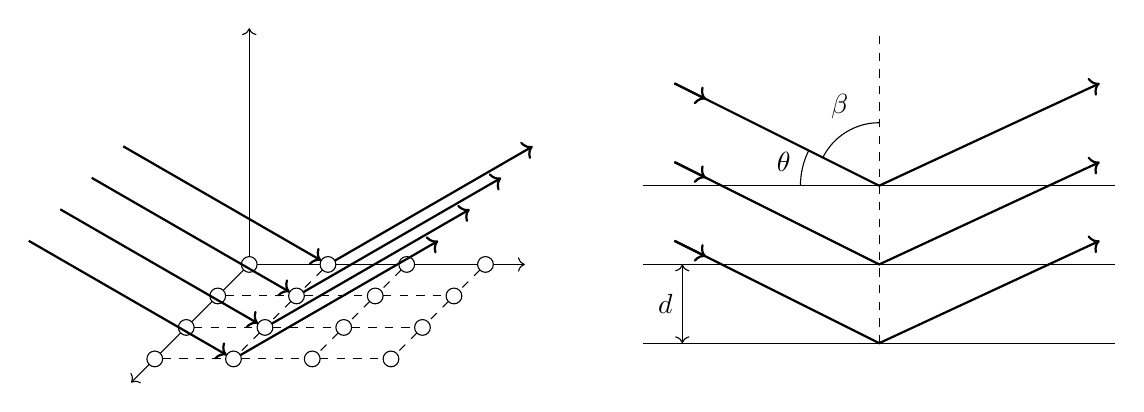
\begin{tikzpicture}
        \draw (-3,0)--(3,0);
        \draw (-3,2)--(3,2);
        \draw (-3,1)--(3,1);
        \draw [dashed] (0,0)--(0,4);
        \draw [<->] (-2.5,0)--(-2.5,1);
        \node [left] at(-2.5,0.5) {$ d $};
        \draw [thick,->] (-2.6,1.3)--(0,0)--(2.8,1.3);
        \draw [thick,->] (-2.6,1.3)--(-2.2,1.1);
        \draw [thick,->] (-2.6,2.3)--(0,1)--(2.8,2.3);
        \draw [thick,->] (-2.6,2.3)--(-2.2,2.1);
        \draw [thick,->] (-2.6,3.3)--(0,2)--(2.8,3.3);
        \draw [thick,->] (-2.6,3.3)--(-2.2,3.1);
        \draw (-1,2) arc (180:154:1);
        \draw (0,2.8) arc (90:154:0.8);
        \node [left] at(-1,2.3) {$\theta$};
        \node at(-0.5,3) {$\beta$};
        
        \draw (-8,1) circle [radius=0.1];
        \draw (-7,1) circle [radius=0.1];
        \draw (-6,1) circle [radius=0.1];
        \draw (-5,1) circle [radius=0.1];
        \draw (-8.4,0.6) circle [radius=0.1];
        \draw (-7.4,0.6) circle [radius=0.1];
        \draw (-6.4,0.6) circle [radius=0.1];
        \draw (-5.4,0.6) circle [radius=0.1];
        \draw (-8.8,0.2) circle [radius=0.1];
        \draw (-7.8,0.2) circle [radius=0.1];
        \draw (-6.8,0.2) circle [radius=0.1];
        \draw (-5.8,0.2) circle [radius=0.1];
        \draw (-9.2,-0.2) circle [radius=0.1];
        \draw (-7.2,-0.2) circle [radius=0.1];
        \draw (-8.2,-0.2) circle [radius=0.1];
        \draw (-6.2,-0.2) circle [radius=0.1];
        \draw [->] (-8,1.1)--(-8,4);
        \draw (-8.07,0.93)--(-8.33,0.67);
        \draw (-8.47,0.53)--(-8.73,0.27);
        \draw (-8.87,0.13)--(-9.13,-0.13);
        \draw [->] (-9.27,-0.27)--(-9.5,-0.5);
        \draw [dashed] (-7.07,0.93)--(-7.33,0.67);
        \draw [dashed] (-7.47,0.53)--(-7.73,0.27);
        \draw [dashed] (-7.87,0.13)--(-8.13,-0.13);
        \draw [dashed] (-6.07,0.93)--(-6.33,0.67);
        \draw [dashed] (-6.47,0.53)--(-6.73,0.27);
        \draw [dashed] (-6.87,0.13)--(-7.13,-0.13);
        \draw [dashed] (-5.07,0.93)--(-5.33,0.67);
        \draw [dashed] (-5.47,0.53)--(-5.73,0.27);
        \draw [dashed] (-5.87,0.13)--(-6.13,-0.13);
        \draw (-7.9,1)--(-7.1,1);
        \draw (-6.9,1)--(-6.1,1);
        \draw (-5.9,1)--(-5.1,1);
        \draw [->] (-4.9,1)--(-4.5,1);
        \draw [dashed] (-8.3,0.6)--(-7.5,0.6);
        \draw [dashed] (-7.3,0.6)--(-6.5,0.6);
        \draw [dashed] (-6.3,0.6)--(-5.5,0.6);
        \draw [dashed] (-8.7,0.2)--(-7.9,0.2);
        \draw [dashed] (-7.7,0.2)--(-6.9,0.2);
        \draw [dashed] (-6.7,0.2)--(-5.9,0.2);
        \draw [dashed] (-9.1,-0.2)--(-8.3,-0.2);
        \draw [dashed] (-8.1,-0.2)--(-7.3,-0.2);
        \draw [dashed] (-7.1,-0.2)--(-6.3,-0.2);
        \draw [thick,->] (-9.60,2.5)--(-7.086,1.05);
        \draw [thick,->] (-10.0,2.1)--(-7.486,0.65);
        \draw [thick,->] (-10.40,1.7)--(-7.886,0.25);
        \draw [thick,->] (-10.80,1.3)--(-8.286,-0.15);
        \draw [thick,->] (-6.91,1.05)--(-4.40,2.5);
        \draw [thick,->] (-7.31,0.65)--(-4.80,2.1);
        \draw [thick,->] (-7.71,0.25)--(-5.20,1.7);
        \draw [thick,->] (-8.11,-0.15)--(-5.60,1.3);
    \end{tikzpicture}
    \caption{同一晶面与不同晶面的散射波示意图}
    \label{fig-scatt}
\end{figure}

处在同一平面上的原子组成一个晶面,它们的散射波相干叠加的结果遵从反射定律。而从间隔为$ d $的相邻两个晶面反射的两束波的程差为$ 2d\sin\theta $,$ \theta $为入射角与晶面的夹角。显然只有满足
\[2d\sin\theta=k\lambda,\qquad k=1,2,3,\cdots\]
才能形成干涉极大。上式称为晶体衍射的布拉格条件,如果改用常用的入射角$ \beta $表示,则布拉格条件可改写为
\[2d\cos\beta=k\lambda,\qquad k=1,2,3,\cdots\]
在本次实验中,已知晶面间距$ d $,通过测量衍射极大时的入射角$ \beta $以求得波长$\lambda$.

由于不同晶面族的曲线不同,晶面间隔也不同,因此当入射波方向及波长固定、晶体取向固定时,不同取向的晶面不能同时满足布拉格条件,甚至没有一族晶面能够满足布拉格条件。为了观察到尽可能多的衍射极大,得到尽可能多的关于晶体结构的信息,在研究晶体结构的实际工作中,采用不同的方法:转动晶体、采用多晶或粉末样品代替单晶、采用包含波长连续变化的X射线代替单一波长的X射线。在本实验中使用入射方向固定、波长单一的微波及单晶模型,从而采用转动晶体模型和接收喇叭的方向来进行对不同晶面的研究。

~\

\section{实验内容}
四实验中所用微波频率一致,均为9.4\,GHz,打开电源后将微波频率设置为9.4\,GHz,并调整实验仪器在桌面上的位置与角度,使得检波器扫描范围能达到$ \pm50^\circ $。

\subsection{实验1:微波的单缝衍射}
转动接收臂使其指针指向载物台的$ 0^\circ $刻线,打开振荡器的电源,转动载物台,使其上的$ 180^\circ $刻线与发射臂的指针一致,调节发生器与接受器姿态,使其正对,微调接收喇叭的朝向,使得在$ \pm20^\circ $处的差异在2\,mV以内。

调节衰减器,使二者正对时接收电表的指示在150\,mV左右。

仪器安装时,按需要先调整单缝衍射板的缝宽,然后把单缝衍射板放到载物台,并使狭缝所在平面与入射方向垂直(微调狭缝角度使得当正对发生器的接收电表示数极大),把单缝的底座固定在载物台上。

转动接收臂,在$ -40^\circ\sim40^\circ $内每隔$ 2^\circ $记下一次接收信号的大小。

为了准确测量波长,需仔细寻找衍射极小的位置。在衍射极小附近,以$ 1^\circ $为步长精扫接收信号的变化。可把衰减器向零处旋转,以增大发射信号的强度,进而提高测量的灵敏度。

根据记录数据,画出单缝衍射强度与衍射角度的关系曲线。并根据微波衍射强度一级极小角度$ \varphi $和缝宽$a$,计算微波波长$\lambda$和其百分误差。

\subsection{实验2:微波的双缝干涉}
放置双缝前,与实验1一样进行实验仪对准确认,使得发生器、接收器分别于$ 180^\circ,0^\circ $处正对,接收信号在$ \pm20^\circ $处强度相当。调节微波发射功率使得在零级极大处接收信号强度在150\,mV左右。

按要求调整双缝干涉板的缝宽均为3.5\,cm。将双缝缝干射板安置在支座上时,应使双缝板平面与载物圆台上$ 90^\circ $指示线一致。在$ -50^\circ\sim50^\circ $范围内,每改变$ 2^\circ $读取一次液晶显示器的读数,并记录下来,然后就可以画出双缝干涉强度与角度的关系曲线。

在两侧零级极大、零级极小、一级极小处以$ 1^\circ $为步长进行精扫,绘制精扫结果图象以确定极值点。

根据微波干涉强度零级极大、零级极小、一级极大角度和缝宽$a$、缝间间隔$ b $,计算微波波长$\lambda$和其百分误差。

\subsection{实验3:迈克尔逊干涉实验}
根据微波的前进方向设置迈克尔逊干涉仪,在极大位置适当调节微波发生功率使其大于100\,mV,便于观察接收信号强度的变化与极小值。将可移动反射板装在一旋转读数机构上后,然后移动旋转读数机构上的手柄,使得可移动反射板移动,测出$ n+1 $个微波极小值,并同时从读数机构上读出可移反射板的移动距离$ L $,则波长满足$ \lambda=\frac{2L}{n} $。

\subsection{实验4:布拉格衍射}
同此前的实验一样,实验进行前需检查发生器和检波器的正对情况。
\subsubsection{ 100 晶面}
将发生器与检波器正对,调节微波发生功率使得接收信号为$ 150\,\mathrm{mV} $左右。安装模型晶体,转动载物圆盘使得发生器位于$ -30^\circ $(即$ 330^\circ $)处,转动接收器使其位于$ 30^\circ $处,即使得入射角与探测方向相对晶面法线对称。将入射角在$ 30^\circ\sim80^\circ $范围内以$ 2^\circ $为步长步进,在相应的探测位置读得并记录接收信号强度。绘制入射角与接收信号强度间的图象。

在信号强度极大值点附近以$ 1^\circ $为步长进行精扫,以确定极大值点对应的入射角。进而求得微波波长$ \lambda=2d\cos\beta $并计算百分误差。

\subsubsection{ 110 晶面}
大致步骤与 100 晶面时一致,不同在于 100 晶面的晶面法线方向为载物圆盘上$ 0^\circ $方向,而 110 晶面的晶面法线方向为载物圆盘上$ 45^\circ $方向。此外粗扫时入射角范围调整为$ 30^\circ\sim70^\circ $,精扫时由于接收信号较弱可适当调节微波发生功率。


\end{document}

% VScode 常用快捷键:

% F2:                       变量重命名
% Ctrl + Enter:             行中换行
% Alt + up/down:            上下移行
% 鼠标中键 + 移动:           快速多光标
% Shift + Alt + up/down:    上下复制
% Ctrl + left/right:        左右跳单词
% Ctrl + Backspace/Delete:  左右删单词    
% Shift + Delete:           删除此行
% Ctrl + J:                 打开 VScode 下栏(输出栏)
% Ctrl + B:                 打开 VScode 左栏(目录栏)
% Ctrl + `:                 打开 VScode 终端栏
% Ctrl + 0:                 定位文件
% Ctrl + Tab:               切换已打开的文件(切标签)
% Ctrl + Shift + P:         打开全局命令(设置)

% Latex 常用快捷键:

% Ctrl + Alt + J:           由代码定位到PDF


